\documentclass[DIN, pagenumber=false, fontsize=11pt, parskip=half]{scrartcl}

\usepackage{amsmath}
\usepackage{amsfonts}
\usepackage{amssymb}
\usepackage{enumitem}
\usepackage[utf8]{inputenc} 
\usepackage[ngerman]{babel} 
\usepackage[T1]{fontenc} 
\usepackage{pgfplots}
\usepackage{xcolor}
\usepackage{listings}
\usepackage{float}
\usepackage{graphicx}
\usepackage{booktabs}
\usepackage{tkz-euclide}
\usepackage{svg}

\definecolor{mygreen}{RGB}{28,172,0} % color values Red, Green, Blue
\definecolor{mylilas}{RGB}{170,55,241}

\tikzstyle{neuron}=[circle,fill=black!25,minimum size=30pt,inner sep=0pt]

\lstset{language=Matlab,%
    %basicstyle=\color{red},
    breaklines=true,%
    morekeywords={matlab2tikz},
    keywordstyle=\color{blue},%
    morekeywords=[2]{1}, keywordstyle=[2]{\color{black}},
    identifierstyle=\color{black},%
    stringstyle=\color{mylilas},
    commentstyle=\color{mygreen},%
    showstringspaces=false,%without this there will be a symbol in the places where there is a space
    numbers=left,%
    numberstyle={\tiny \color{black}},% size of the numbers
    numbersep=9pt, % this defines how far the numbers are from the text
    emph=[1]{for,end,break},emphstyle=[1]\color{red}, %some words to emphasise
    %emph=[2]{word1,word2}, emphstyle=[2]{style},    
}

\title{Einführung in die Neuroinformatik}
\author{Tim Luchterhand, Paul Nykiel (Gruppe P)}

\begin{document}
    \maketitle
    \section{Cross Entropy}
    \begin{enumerate}
        \item Man kann und darf keine Aussage über die \glqq{}Schwere\grqq{} des Fehlers machen. Nur weil für die Eingabe $x_1$ um \glqq{}zwei Klassen\grqq{} vom Traininssignal abweicht, ist die Klassifikation nicht schlechter als für $x_2$, welches nur um eine Klasse abweicht.
		\item Wurde erfolgreich gelesen $\surd$
		\item
			\begin{enumerate}[label=(\alph*)]
				\item
					\begin{eqnarray*}
							H_A(B) &=& \sum_x{B(x)\cdot \log_2\left(\frac{1}{A(x)}\right)} \\
							&=& \frac{1}{2} \log_2(8) + \frac{1}{4} \log_2(2) + \frac{1}{8} \log_2(4) + \frac{1}{8} \log_2(8) \\
							&=&\frac{19}{8}
					\end{eqnarray*}
				\item
					\begin{eqnarray*}
							H_B(A) &=& \sum_x{A(x)\cdot \log_2\left(\frac{1}{B(x)}\right)} \\
							&=& \frac{1}{8} \log_2(2) + \frac{1}{2} \log_2(4) + \frac{1}{4} \log_2(8) + \frac{1}{8} \log_2(8) \\
							&=&\frac{9}{4}
					\end{eqnarray*}
				\item
					\begin{eqnarray*}
							H_B(B) &=& \sum_x{B(x)\cdot \log_2\left(\frac{1}{B(x)}\right)} \\
							&=& \frac{1}{2} \log_2(2) + \frac{1}{4} \log_2(4) + 2 \cdot \frac{1}{8} \log_2(8) \\
							&=&\frac{7}{4}
					\end{eqnarray*}
				\item
					\begin{eqnarray*}
							D_A(B) &=& H_A(B) - H(B) = \frac{19}{8} - \frac{7}{4} = \frac{5}{4} \\
							D_B(B) &=& H_B(B) - H(B) = H(b) - H(B) = 0 \\
							D_B(A) &=& H_B(A) - H(A) = \frac{9}{4} - \frac{7}{4} = \frac{1}{2} 
					\end{eqnarray*}
			\end{enumerate}
		\item Es gilt:
			\begin{equation*}
					D_Q(P) = H_Q(P) - H(P) \geq H(P) - H(P) = 0 \ \forall \ P,Q \in X
			\end{equation*}
			denn $H_Q(P)\geq H(P)$ und $H(P) < 0 \ \forall \ P$

			Außerdem gilt:
			\begin{equation*}
					D_Q(Q) = H_Q(Q) - H(Q) = H(Q) - H(Q) = 0 \ \forall \ Q \in X
			\end{equation*}
		\item
			\begin{enumerate}[label=(\alph*)]
				\item Das Minnimum muss auftreten, wenn $C=B$
						\begin{equation*}
								\Rightarrow t \cdot \frac{3}{4} \overset{!}{=} \frac{1}{2} \Rightarrow t = \frac{2}{3}
						\end{equation*}
				\item $ $ 
                    \lstinputlisting{b06a01.m}
                    \lstinputlisting{C.m}

                    \begin{figure}[H]
                        \centering
                        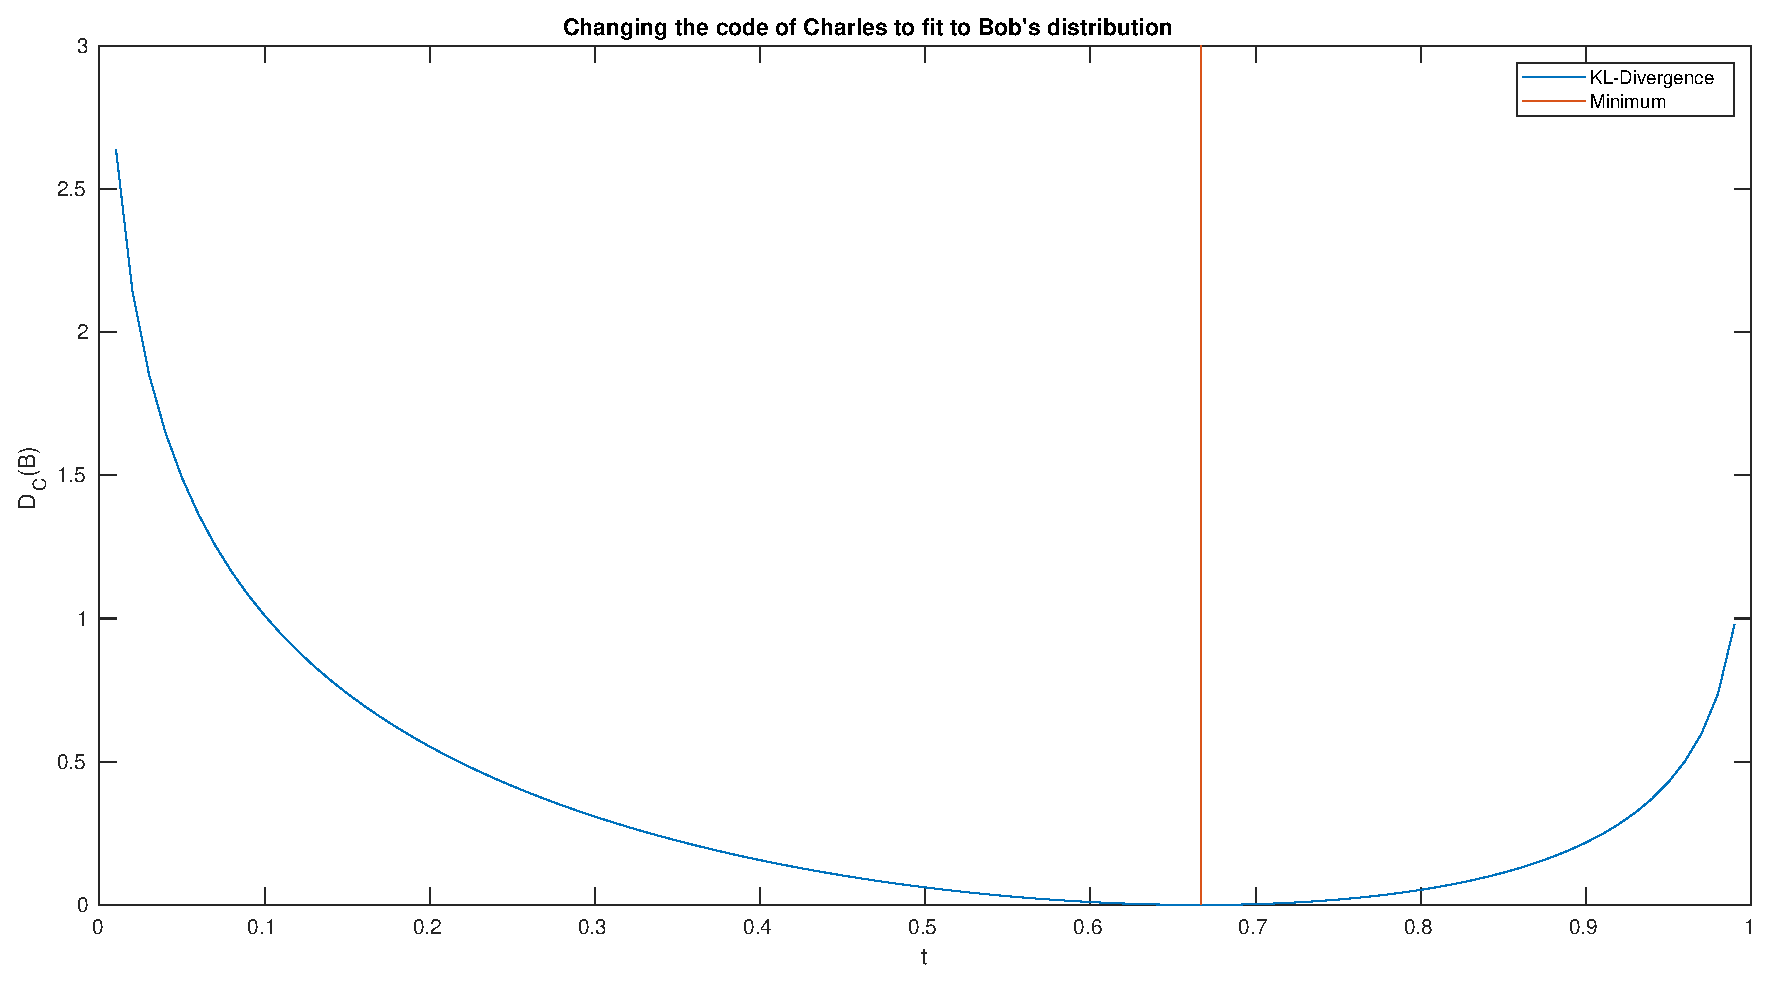
\includegraphics[width=\textwidth]{plot.eps}
                        \caption{Ergebnis des Matlab Skripts}
                    \end{figure}
			\end{enumerate}
    \end{enumerate} 
	\section{Cross Entropy als Kostenfunktion}
	\begin{enumerate}
		\item
			\begin{enumerate}[label=(\alph*)]
				\item
					\begin{equation*}
							y_i > 0 \ \forall i \text{, da } e^{c\cdot u_l} > 0 \ \forall c, u_l \in \mathbb{R}
					\end{equation*}
					und 
					\begin{eqnarray*}
							\sum_{i=1}^{n}{y_i} &=& \sum_{i=1}^{n}{\left( e^{c\cdot u_i} \cdot \dfrac{1}{\sum_{j=1}^{n}{e^{c\cdot u_j}}} \right)} \\
							&=& \dfrac{\sum_{i=1}^{n}{e^{c\cdot u_i}}} {\sum_{j=1}^{n}{e^{c\cdot u_j}}} = 1
					\end{eqnarray*}
				\item
					\begin{eqnarray*}
							y_1 &=& \dfrac{e^{c \cdot u_1}}{e^{c \cdot u_1} + e^{c \cdot u_2} + e^{c \cdot u_3}} \\
							&=& \dfrac{e^{-c \cdot u_1}}{e^{-c \cdot u_1}} \cdot \frac{e^{c \cdot u_1}}{e^{c \cdot u_1} + e^{c \cdot u_2} + e^{c \cdot u_3}} \\
							&=& \dfrac{1}{1 + e^{c \cdot (u_2 - u_1)} + e^{c \cdot (u_3 - u_1)}}
					\end{eqnarray*}
				\item
					Fall $u_1 > u_2 > u_3$:
					\begin{equation*}
							\lim_{c\rightarrow \infty}y_1 = 1
					\end{equation*}
					Fall $u_2 > u_1 > u_3$:
					\begin{equation*}
							\lim_{c\rightarrow \infty}y_1 = 0
					\end{equation*}
					Fall $u_2 > u_3 > u_1$:
					\begin{equation*}
							\lim_{c\rightarrow \infty}y_1 = 0
					\end{equation*}
				\item
					Für $c \rightarrow \infty$ konvergiert die Netzwerkausgabe gegen einen der Trainingsvektoren. D.h. $y_i = 0 \  \forall i \neq k \wedge y_k = 1$
				\item
					Fall $c>0$: 

					Alle $y_i$ werden gegenüber dem $y_k$, für welches $u_k > u_i \ \forall i\neq k$ gilt, gedämpft.

					Fall $c < 0$:

					Alle $y_i$ werden gegenüber dem $y_k$, für welches $u_k < u_i \ \forall i\neq k$ gilt, gedämpft.

					Fall $c = 0$:

					Alle $y_i$ haben den gleich Wert $y_i = \frac{1}{n}$
			\end{enumerate}
		\item
			\begin{equation*}
					E = -t_1 \log(y_1(u_1(w_1), u_2(w_2))) -t_2 \log(y_2(u_1(w_1), u_2(w_2)))
			\end{equation*}
			\begin{enumerate}[label=(\alph*)]
				\item
					\begin{eqnarray*}
							\frac{\partial E}{\partial y_1} = -t_1 \cdot \frac{1}{y_1} \\
							\frac{\partial E}{\partial y_2} = -t_2 \cdot \frac{1}{y_2}
					\end{eqnarray*}
				\item
					\begin{eqnarray*}
							\frac{\partial y_1}{\partial u_2} &=& \frac{\partial}{\partial u_2}\left( \dfrac{e^{u_1}}{e^{u_1} + e^{u_2}} \right) = 
							e^{u_1}\left( -\dfrac{e^{u_2}}{(e^{u_1} + e^{u_2})^2} \right) \\
							&=&-\dfrac{e^{u_1}}{e^{u_1} + e^{u_2}} \cdot \dfrac{e^{u_2}}{e^{u_1} + e^{u_2}} \\
							&=& -y_1 \cdot y_2 \\
							\frac{\partial y_2}{\partial u_2} &=& y_2 + e^{u_2} \cdot \left( -\dfrac{e^{u_2}}{(e^{u_1} + e^{u_2})^2}  \right) \\
							&=& y_2 + \dfrac{e^{u_2}}{e^{u_1} + e^{u_2}} \cdot \left( -\frac{e^{u_2}}{e^{u_1} + e^{u_2}}  \right) \\
							&=& y_2 + y_2(-y_2) = y_2 (1-y_2)
					\end{eqnarray*}
				\item
					\begin{eqnarray*}
							u_2 &=& w_2 x + b \\
							\Rightarrow \frac{\partial u_2}{\partial w_2} &=& x
					\end{eqnarray*}
				\item
					\begin{eqnarray*}
							\frac{\partial E}{\partial w_2} &=& \frac{\partial E}{\partial y_1} \frac{\partial y_1}{\partial u_2} \frac{\partial u_2}{\partial w_2} + 
							\frac{\partial E}{\partial y_2} \frac{\partial y_2}{\partial u_2} \frac{\partial u_2}{\partial w_2}  \\
							&=& \frac{-t_1}{y_1} \cdot (-y_1 y_2) \cdot x + \frac{-t_2}{y_2} \cdot y_2(1-y_2)x \\
							&=& x \cdot (t_1 y_2 - t_2(1-y_2)) \\
							&=& x \cdot (y_2 \cdot (t_1 + t_2) - t_2) = x \cdot (y_2 - t_2)
					\end{eqnarray*}
				\item
                    Im Gegensatz zur Quadratischen-Fehlerfunktion ist diese Fehlerfunktion nicht quadratisch. Außerdem wird die Netzwerkeingabe berücksichtigt.
			\end{enumerate}
	\end{enumerate}
\end{document}
